\documentclass[11pt,letterpaper]{article}

\usepackage[T1]{fontenc}
\usepackage[utf8]{inputenc}
\usepackage{lmodern}
\usepackage{microtype}
\usepackage[margin=1in]{geometry}
\usepackage{amsmath,amssymb}
\usepackage{booktabs,longtable,tabularx,array,multirow}
\usepackage{graphicx}
\usepackage[dvipsnames]{xcolor}
\usepackage{enumitem}
\usepackage{natbib}
\usepackage{tikz}
\usetikzlibrary{arrows.meta,positioning,fit,shapes.geometric}
\usepackage[hidelinks]{hyperref}
\usepackage[nameinlink,noabbrev]{cleveref}
\usepackage{authblk}

\graphicspath{{figures/}}
\setlist{nosep,leftmargin=*}
\setlength{\parskip}{0.35em}
\setlength{\parindent}{0pt}
\renewcommand{\arraystretch}{1.16}
\newcolumntype{Y}{>{\raggedright\arraybackslash}X}
\newcolumntype{P}[1]{>{\raggedright\arraybackslash}p{#1}}

\input{generated/generated_numbers.tex}

\title{\textbf{SynTrustBench: A Trustworthiness Evidence Standard for Synthetic Clinical Data}\\
\large A Systematic Evidence Synthesis, Benchmark Specification, and Pilot Audit}

\author[1]{Neeam Shahriar Hayder}
\author[2]{Iram Wajahat}
\author[1]{Syed Ahmad Chan Bukhari\thanks{Corresponding author: \href{mailto:bukharis@stjohns.edu}{bukharis@stjohns.edu}}}
\affil[1]{Division of Computer Science, Mathematics and Science, St. John's University, New York, NY 11439, USA}
\affil[2]{College of Pharmacy and Health Sciences, St. John's University, New York, NY 11439, USA}
\date{Version 0.1.0 --- July 2026}

\begin{document}
\maketitle

\begin{abstract}
Synthetic clinical data are often called trustworthy after passing a small collection of realism tests. That conclusion is too strong. A dataset can reproduce marginal distributions while leaking training membership, erasing rare subgroups, failing on real patients, or proving impossible to reproduce. Existing benchmarks, reviews, and scorecards make major progress, but they do not provide a common cross-modality method for auditing whether a published trust claim is supported by complete, reproducible evidence across trust dimensions.

We introduce \textbf{SynTrustBench}, a cross-modality evidence standard for synthetic clinical data. Version 0.1.0 has two parts: (i) a benchmark specification covering fidelity, clinical utility/validity, privacy, equity, and robustness/generalization; and (ii) a source-level pilot audit of \CorpusN{} reports published from 2018 through 2025. Each report receives a five-element Evidence Maturity Profile from 0 to 4 and a separate evaluability gate. The dimensions are deliberately non-compensable: strong fidelity cannot cancel absent privacy or equity evidence. The accompanying benchmark card records datasets, versions, splits, threat models, uncertainty, subgroup definitions, code, and failure conditions in machine-readable form.

The audit also corrects material errors in the inherited review corpus, including generator/framework confusion, differential-privacy claims unsupported by the primary source, and mismatched bibliographic identifiers. In the corrected corpus, \PrivacyN{}/\CorpusN{} reports (\PrivacyNPct) perform a quantitative privacy evaluation, \FormalDPN{}/\CorpusN{} (\FormalDPNPct) meet our source-documentation threshold for a formal differential-privacy claim, and \EpsilonN{}/\CorpusN{} (\EpsilonNPct) report a numeric privacy budget. Equity and robustness evidence remain uneven: \FairnessN{}/\CorpusN{} (\FairnessNPct) and \RobustnessN{}/\CorpusN{} (\RobustnessNPct), respectively. We do not construct a literature-derived model leaderboard, because reported values are not comparable across datasets, cohorts, tasks, splits, and threat models. Direct model ranking is reserved for a later controlled-execution track. SynTrustBench therefore benchmarks the maturity of evidence first---the minimum defensible step before benchmarking model performance.
\end{abstract}

\textbf{Keywords:} synthetic clinical data; benchmark; trustworthiness; differential privacy; clinical utility; fairness; robustness; evidence maturity

\section{Introduction}

Synthetic clinical data sit inside an unusually difficult promise. They are expected to look like patient data, preserve the conclusions of clinical analyses, support useful models, protect the people whose records trained the generator, and represent groups that the original health system may already have underserved. These goals are related, but they are not interchangeable. A realistic synthetic record can still be a near-copy. A private generator can still erase rare disease patterns. A model trained on synthetic data can preserve average discrimination while becoming miscalibrated for the patients most likely to be harmed.

The literature often compresses these questions into the word \emph{quality}. That compression creates two problems. First, evaluation becomes a menu: authors select convenient metrics and a favorable subset is taken as evidence of trustworthiness. Second, results that were produced under different cohorts, tasks, splits, model-selection procedures, and attackers are placed side by side as if they measured the same object. Neither practice supports a defensible model ranking.

Several strong benchmarks already address parts of this problem. Synthcity provides an extensible execution framework for synthetic-data generators \citep{qian2023synthcity}. SynthEHRella, CLOVER, and recent large tabular evaluations compare systems under structured-EHR protocols \citep{chen2025synthehrella,qi2026clover,nanevski2026quality}. CheXGenBench does the same for chest radiographs \citep{dutt2026chexgenbench}. Kaabachi et al. review privacy, utility, and fairness metrics across 73 reports; the SMD Scorecard proposes seven cross-modal criteria; and TRUST-SD audits translation readiness and governance reporting in tabular clinical applications \citep{kaabachi2025privacyutility,zamzmi2025scorecard,castagno2026trustsd}. The gap is therefore not ``the first benchmark combining fidelity, utility, and privacy,'' the first scorecard, or the first cross-modal framework. Those claims would be false.

The remaining gap concerns the \emph{unit and gate of evaluation}. Before asking which generator wins, we need to ask whether the evidence offered for each trust claim is complete, interpretable, reproducible, and comparable. SynTrustBench operationalizes a report-level, primary-source audit and prevents incomplete reports from entering comparative scoring through a separate evaluability gate.

This paper makes four contributions:

\begin{enumerate}
    \item \textbf{An evidence-gated benchmark specification.} We define required inputs, metrics, threat models, uncertainty, subgroup analyses, failure conditions, and reporting fields for five trustworthiness dimensions.
    \item \textbf{A non-compensable Evidence Maturity Profile.} Each dimension is rated separately from 0 to 4, while reproducibility is enforced through an evaluability gate. No weighted average can hide a missing privacy or equity evaluation.
    \item \textbf{A corrected, source-linked pilot corpus.} We re-audit \CorpusN{} included reports at the primary-source level, distinguish reports from peer-reviewed studies, separate evaluation frameworks from generators, and regenerate every count from the annotation file.
    \item \textbf{A reusable artifact.} We provide the annotation schema, codebook, benchmark card, validation code, generated tables, and audit log as part of the preprint source package.
\end{enumerate}

Version 0.1.0 is intentionally a Phase 1 release. It contains no new model training and no empirical performance leaderboard. That boundary is not cosmetic: without common data access, frozen splits, consistent threats, and repeated runs, a cross-paper leaderboard would replace missing evidence with false precision.

\section{Related Benchmarks and the Remaining Gap}
\label{sec:related}

\Cref{tab:comparators} separates three kinds of prior work: execution suites that rerun models, domain-specific empirical comparisons, and reporting or governance guidance. This distinction matters because they answer different questions.

\begingroup
\small
\setlength{\tabcolsep}{3.5pt}
\begin{longtable}{P{2.2cm}P{3.5cm}P{2.1cm}P{6.5cm}}
\caption{Closest benchmarks and standards. The mode column distinguishes controlled model execution from reviews, scorecards, report audits, and normative guidance. Relative scope statements are our interpretation of the cited primary sources.}\label{tab:comparators}\\
\toprule
Resource & Primary object and modality & Mode & Main distinction \\
\midrule
\endfirsthead
\toprule
Resource & Primary object and modality & Mode & Main distinction \\
\midrule
\endhead
Synthcity \citep{qian2023synthcity} & Generator library; primarily tabular, with temporal and survival support & Controlled execution & Extensible execution engine; not a cross-modality audit of evidence reported in clinical papers. \\
SynthEHRella \citep{chen2025synthehrella} & Model benchmark; phenotype-aggregated EHR & Controlled execution & Structured-EHR comparison with privacy and transportability tests under a bounded protocol. \\
CheXGen\allowbreak Bench \citep{dutt2026chexgenbench} & Model benchmark; chest radiographs & Controlled execution & Deep imaging protocol on a common dataset; does not audit published claims across modalities. \\
CLOVER \citep{qi2026clover} & Utility--privacy benchmark; tabular EHR & Controlled execution & Compares generators and privacy regimes directly; it does not provide a report-level evidence gate. \\
PLOS benchmark \citep{nanevski2026quality} & Metric and model comparison; single-table health data & Controlled execution & Broad tabular metric matrix; limited clinical-validity, robustness, and reporting coverage. \\
Imbalance framework \citep{kim2026imbalanced} & Prevalence-stratified structured-EHR evaluation & Controlled execution & Makes rare-outcome behavior visible within a narrower cohort, model-family, and modality scope. \\
Kaabachi review \citep{kaabachi2025privacyutility} & Metric taxonomy; tabular health data & Review and audit & Audits 73 reports for utility, privacy, and fairness metrics, without a per-report maturity profile or evaluability gate. \\
SMD Scorecard \citep{zamzmi2025scorecard} & Seven-criterion dataset scorecard; cross-modal & Scorecard & Closest cross-modal scorecard; it does not supply a source-audited report corpus or gate comparative use. \\
TRUST-SD \citep{castagno2026trustsd} & Governance and readiness; tabular clinical applications & Report audit & Closest conceptual comparator; SynTrustBench adds cross-modality, machine-readable source linkage, robustness, and an explicit gate. \\
NIST SP 800-226 \citep{near2025nist} & Differential-privacy guarantee evaluation; domain-general & Normative standard & Privacy foundation for formal claims, rather than a full synthetic-clinical benchmark. \\
\bottomrule
\end{longtable}
\endgroup

Execution benchmarks produce model-level measurements under bounded data settings. SynthEHRella compares seven methods and two baselines on MIMIC-III and MIMIC-IV phenotype representations; CheXGenBench evaluates eleven text-to-image architectures with more than twenty metrics; and CLOVER compares eight tabular approaches over MIMIC-III, eICU, and multiple differential-privacy regimes \citep{chen2025synthehrella,dutt2026chexgenbench,qi2026clover}. These are the right tools for deciding how a runnable system behaves under their protocol.

Reviews and reporting frameworks ask a different question. Earlier syntheses cataloged generation methods and the heterogeneity of tabular evaluation \citep{chen2021syntheticmedicine,hernandez2022tabularreview}. Kaabachi et al. systematized utility, privacy, and fairness evidence across 73 reports, while the SMD Scorecard proposed Congruence, Coverage, Constraint, Completeness, Compliance, Comprehension, and Consistency as cross-modal criteria \citep{kaabachi2025privacyutility,zamzmi2025scorecard}. TRUST-SD then reviewed 37 peer-reviewed tabular clinical applications and proposed a preliminary seven-domain readiness checklist \citep{castagno2026trustsd}. NIST SP 800-226 provides detailed guidance for evaluating differential-privacy guarantees \citep{near2025nist}. SynTrustBench complements these resources through a primary-source-audited report corpus, dimension-wise maturity anchors, and an explicit gate that blocks comparative scoring when essential evidence is missing.

\section{Systematic Evidence-Synthesis and Audit Methods}
\label{sec:methods}

\subsection{Frozen pilot corpus and claim boundary}

The Phase 1 audit begins with the 30-report corpus assembled for the preceding review. Retained project records describe searches of PubMed, IEEE Xplore, and the ACM Digital Library for reports published from January 2018 through December 2025, followed by backward citation tracking. They record 184 candidate records, 63 duplicates, 121 title/abstract records, 51 full texts, and 30 included reports. However, the retained source subtotals (30 PubMed, 69 IEEE Xplore, 76 ACM, and six backward-citation records) sum to 181 rather than 184, and the exact historical line-by-line search exports were not retained. We use PRISMA 2020 terminology to describe the recoverable inherited flow; the missing records preclude a complete PRISMA reconstruction or checklist claim \citep{page2021prisma}.

We do not silently repair that discrepancy. Version 0.1.0 freezes the 30 included reports as a \emph{pilot audit corpus}; descriptive percentages refer to that corpus, not to an exhaustive census of the field. \Cref{app:search} gives reproducible reconstructed search syntax for the planned update, clearly labeled as a reconstruction rather than the missing historical log. Studies published in 2026 are used to position the benchmark but are not added to the frozen audit denominator.

\subsection{Eligibility and report types}

The audit includes full reports that (i) generate synthetic clinical data or empirically evaluate generators on clinical data; (ii) evaluate at least one of statistical/clinical fidelity, downstream utility, or privacy; and (iii) report quantitative results. We exclude non-healthcare applications, purely conceptual proposals without an empirical clinical evaluation, abstracts without a full report, and data-augmentation studies that do not generate or evaluate a synthetic clinical modality.

This rule resolves the inherited contradiction between an ``at least one fidelity, privacy, or utility dimension'' inclusion rule and a footnote that appeared to require privacy from every report. Privacy is \emph{not} an eligibility condition. Its absence is an audit result. We use \emph{included reports} rather than \emph{30 peer-reviewed studies}: the corpus contains preprints and theses alongside journal and conference papers.

\subsection{Primary-source re-extraction}

The annotation unit is the report. We reviewed the full primary source and, when available, its official supplement or repository. Publisher and proceedings pages establish bibliographic status; secondary reviews do not establish technical fields. For each report we extracted publication type, review status, task scope, generated modality, architecture family, evaluated systems, datasets and versions, data/code access, fidelity and clinical-validity tests, held-out utility, privacy tests and threats, formal-DP mechanism and parameters, equity/subgroup analysis, robustness, external validation, seeds, uncertainty, and reproducibility fields. The complete schema contains 62 columns and is provided with the source package.

We used three missingness states. \texttt{NR} means that the primary source did not report the field. \texttt{NA} means that the field is structurally inapplicable. ``No'' is used only when the report allows a negative determination. De-identification, restricted access, or a statement of HIPAA/GDPR alignment does not count as a privacy evaluation. A model counts as formally differentially private only when the evaluated pipeline provides an algorithm-level guarantee with an identifiable DP mechanism; comparison with a DP baseline or the addition of unaccounted gradient noise is insufficient.

Every material correction is recorded as old value, new value, rationale, primary source, date, and adjudication status. The original spreadsheet is preserved in a dated, unchanged snapshot.

The five dimensions came from the preceding evidence synthesis. We translated them into operational anchors before the final code-generated rescore, using the closest empirical benchmarks, reporting frameworks, and NIST privacy guidance to sharpen dimension-specific criteria \citep{kaabachi2025privacyutility,zamzmi2025scorecard,castagno2026trustsd,near2025nist}. These v0.1 anchors are provisional author specifications. They have not undergone Delphi consensus, formal content-validity assessment, or prospective calibration against controlled model runs.

\subsection{Evidence Maturity Profile}

SynTrustBench rates the maturity of the \emph{evidence}, not whether the result favors the model. Each dimension receives an ordinal level:

\begin{description}[style=nextline]
    \item[0 --- Not evaluated.] No quantitative evidence for the dimension.
    \item[1 --- Descriptive or surrogate.] One visual, descriptive, proxy, or weakly matched test.
    \item[2 --- Appropriate held-out or multi-metric evidence.] Multiple complementary tests, or one well-designed held-out/attack evaluation with enough detail to interpret.
    \item[3 --- Stress-tested evidence.] Adversarial, subgroup, repeated, clinically reviewed, or externally validated evidence, with uncertainty where applicable.
    \item[4 --- Independently reproducible or formally complete.] Level 3 evidence with enough dimension-specific artifacts to reproduce the claim independently, or source documentation that meets the benchmark threshold for a complete formal guarantee where that is the relevant standard.
\end{description}

Level 4 and the gate intentionally overlap but answer different questions. Level 4 asks whether one dimension's evidence is independently reproducible; the gate asks whether the report's overall protocol clears the minimum prerequisites for comparative use. A report can pass the gate without reaching Level 4 in any dimension.

Dimension-specific anchors are in \Cref{tab:maturity}. A separate evaluability gate is \emph{Pass}, \emph{Conditional}, or \emph{Fail}. A Pass requires the model/version, cohort/preprocessing, split logic, metric implementation, run configuration, code, and a lawful data-access route or fully specified substitute. A future performance submission cannot enter a comparative SynTrust leaderboard unless the gate is Pass.

\subsection{Reviewer status and analysis}

The pilot annotations were primary-coded and then subjected to a separate automated source-checking pass that flagged conflicts for human adjudication. This automated assistance is not a substitute for a second human reviewer. Human double-coding of all privacy, DP, equity, ambiguous task fields, and a random sample of remaining fields was not complete at the time of version 0.1.0; therefore, we report no Cohen's $\kappa$ or Gwet's AC1. The released sheet marks every row as awaiting human double-code. This is a limitation of the pilot, not a statistic to be invented.

All counts, percentages, maturity tables, and figures are generated from \texttt{study\_annotations.csv}. The validation script asserts a 30-report denominator, checks title and citation-key uniqueness, rejects impossible DP combinations, and prevents a benchmark framework from being labeled as its baseline architecture. We do not pool effect sizes or compare published performance values across heterogeneous tasks.

\section{SynTrustBench Design}
\label{sec:design}

\subsection{Two tracks, one explicit boundary}

\begin{figure*}[t]
\centering
\resizebox{\textwidth}{!}{%
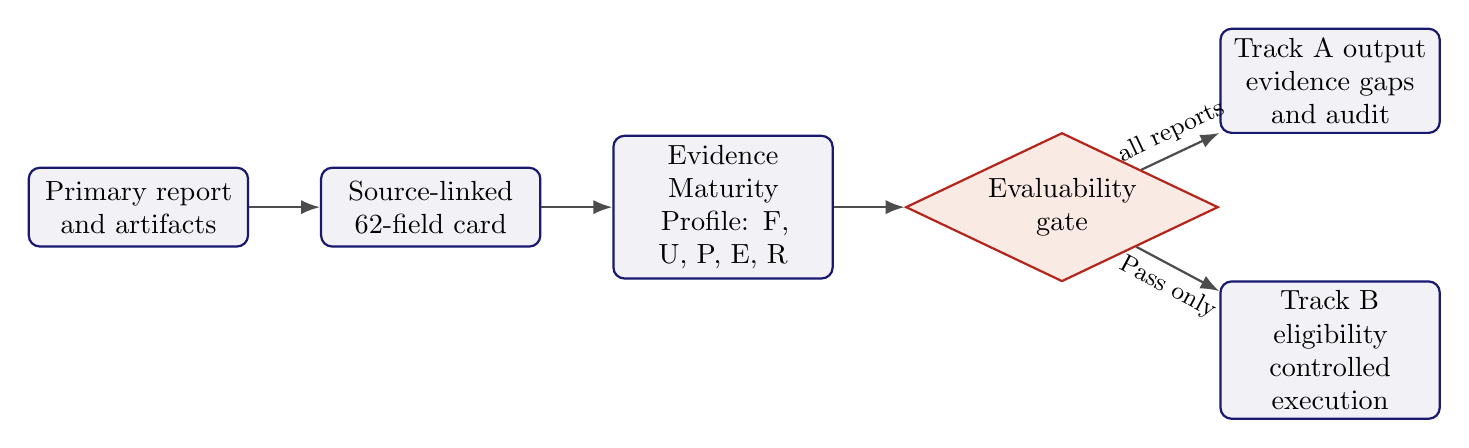
\begin{tikzpicture}[
    node distance=0.75cm and 0.9cm,
    box/.style={rounded corners, draw=MidnightBlue, thick, fill=MidnightBlue!6, align=center, minimum height=1.0cm, text width=2.55cm},
    gate/.style={diamond, draw=BrickRed, thick, fill=BrickRed!7, align=center, aspect=2.1, inner sep=1.5pt, text width=2.1cm},
    arrow/.style={-{Latex[length=2.4mm]}, thick, draw=black!70}
]
\node[box] (report) {Primary report\\and artifacts};
\node[box, right=of report] (extract) {Source-linked\\62-field card};
\node[box, right=of extract] (profile) {Evidence Maturity\\Profile: F, U, P, E, R};
\node[gate, right=of profile] (gate) {Evaluability\\gate};
\node[box, above right=0.45cm and 1.0cm of gate] (audit) {Track A output\\evidence gaps and audit};
\node[box, below right=0.45cm and 1.0cm of gate] (execute) {Track B eligibility\\controlled execution};
\draw[arrow] (report) -- (extract);
\draw[arrow] (extract) -- (profile);
\draw[arrow] (profile) -- (gate);
\draw[arrow] (gate) -- node[above,sloped,font=\small]{all reports} (audit);
\draw[arrow] (gate) -- node[below,sloped,font=\small]{Pass only} (execute);
\end{tikzpicture}%
}
\caption{SynTrustBench separates the evidence audit implemented in Phase 1 from controlled model execution planned for Phase 2. The gate is not averaged into the profile.}
\label{fig:pipeline}
\end{figure*}

Track A evaluates a report and its artifacts. Its outputs are a source-linked benchmark card, a five-dimensional profile, an evaluability gate, and explicit missing-evidence flags. Track B will execute models under a common protocol. A Track B result is identified by the tuple

\begin{equation}
\{v, m, d, c, t, s, g, e\},
\end{equation}

where $v$ is benchmark version, $m$ modality protocol, $d$ dataset version, $c$ cohort definition, $t$ clinical task, $s$ split hash, $g$ generator version, and $e$ evaluation-code version. Results with different tuples must not share a leaderboard.

\subsection{Five non-compensable dimensions}

\textbf{Fidelity} asks whether the synthetic output preserves distributions, dependencies, support, and clinically meaningful structure. \textbf{Clinical utility/validity} asks whether synthetic-data training or analysis preserves decisions on real held-out patients, including calibration and clinical agreement where relevant. \textbf{Privacy} asks what a declared attacker can infer and whether any formal guarantee is completely documented. \textbf{Equity} asks whether fidelity, utility, and disclosure risk are preserved across protected and clinically important subgroups. \textbf{Robustness/generalization} asks whether conclusions survive seeds, perturbations, missingness, site/time shift, and external validation. Safety failures remain explicit blocking flags in the benchmark card; a favorable utility result cannot cancel a prespecified safety failure.

We report the vector
\begin{equation}
\mathrm{EMP} = [F, U, P, E, R], \qquad F,U,P,E,R \in \{0,1,2,3,4\},
\end{equation}
plus the evaluability gate. Version 0.1.0 defines no weighted total. This is deliberate. An arithmetic score such as 25/25/25/15/10 allows excellent realism to cancel a missing privacy test. Trust dimensions are constraints before they are preferences.

\subsection{Benchmark card}

The machine-readable card records intended and prohibited uses; system and data versions; cohort and split hashes; seeds and failed runs; uncertainty; all five evidence sections; DP adjacency, mechanism, $\epsilon$, $\delta$, and accountant; subgroup definitions and denominators; failure flags; artifact links; and adjudication status. Empty fields remain visible as missing evidence.

\section{Provisional Benchmark Tasks and Recommended Metrics}
\label{sec:tasks}

\begin{table*}[t]
\centering
\caption{Provisional v0.1 recommended evaluation bundle. These criteria require prospective calibration and expert validation; modality-specific alternatives are expected when a generic metric is clinically inappropriate.}
\label{tab:bundle}
\small
\setlength{\tabcolsep}{4pt}
\begin{tabular}{P{2.8cm}P{4.3cm}P{4.0cm}P{4.0cm}}
\toprule
Dimension & Required evidence & Required reporting & Failure condition \\
\midrule
Fidelity & Type-appropriate marginals; dependency/structure; support coverage; rare-pattern analysis & Metric direction, real/synthetic sample sizes, uncertainty, clinical constraints & Clinically impossible records or severe support collapse \\
Clinical utility/\allowbreak validity & Frozen TSTR on real data; TRTR reference; discrimination and calibration when relevant; structured clinical review by modality & Task, split, prevalence, model selection, seeds, uncertainty, non-inferiority margin & Prespecified unsafe disagreement or material loss beyond margin \\
Privacy & Declared threat model; MIA at low FPR; attribute/reconstruction test when applicable; complete DP accounting if claimed & Attacker access and auxiliary data; member/non-member design; $\epsilon$, $\delta$, adjacency, accountant, tuning cost & Attack above risk threshold; missing threat; incomplete DP claim \\
Equity & Subgroup denominators; subgroup fidelity, utility, and privacy; uncertainty & Protected/clinical attributes, intersection rules, small-cell handling & Any subgroup below a floor or unsupported due to sample size \\
Robustness/\allowbreak generalization & At least five seeds; one prespecified stress test; external/temporal validation when available & Failures, dispersion, shift definition, external cohort differences & Conclusion reverses under a prespecified stressor \\
\bottomrule
\end{tabular}
\end{table*}

For structured EHRs, a minimum fidelity bundle should combine type-appropriate marginal distances, mixed-type dependency preservation, and support coverage. Utility should use TSTR on a frozen real test set with AUPRC for imbalanced outcomes and calibration for risk predictions. For time series, the bundle adds autocorrelation, cross-correlation, event timing, missingness, and sequence-length preservation. For images, generic natural-image FID cannot stand alone; anatomy/pathology consistency, diversity, a real held-out task, expert assessment, and patient-level privacy tests are needed. For clinical text, ROUGE cannot stand alone; the bundle adds clinical concept consistency, factuality, contradiction/hallucination, temporal and medication coherence, and a realistic leakage test. Multimodal submissions must also test cross-modal consistency and linkage privacy.

For the future controlled-execution track, v0.1 recommends at least five seeds and reports all failed runs; this is a provisional default, not a universal sufficiency threshold. The recommended privacy operating point is true-positive rate at 1\% false-positive rate, accompanied by the complete curve and uncertainty. Average attack AUROC can conceal a small group of highly exposed patients \citep{carlini2022membership}. Results should therefore be stratified by protected attributes and clinically meaningful rarity when sample size permits. DP claims follow NIST SP 800-226 and must include every privacy-consuming step \citep{near2025nist}.

\section{Pilot Evidence Audit}
\label{sec:results}

\subsection{Corpus composition after correction}

The corrected corpus contains \CorpusN{} included reports across tabular EHR, clinical time series, medical imaging, and clinical text. Publication type is not collapsed into ``peer reviewed'': journal and proceedings papers, preprints, and theses are reported separately. Likewise, reports that introduce an evaluation framework are separated from reports that introduce a generator.

Several corrections changed the paper's core claims. CorGAN performs empirical disclosure-risk analyses but does not implement or report formal DP \citep{torfi2020corgan}. PPGAN evaluates membership inference and compares against a DP baseline, but the evaluated PPGAN pipeline does not report DP-SGD, $\epsilon$, $\delta$, or an accountant \citep{ashrafi2023ppgan}. SynQP is an evaluation framework using generators as test cases, not itself a GAN \citep{hu2025synqp}. Statements that data were de-identified or ``HIPAA/GDPR aligned'' are governance descriptions, not privacy tests. The source audit also replaces mismatched identifiers where the bibliography pointed to a different work than the coded row.

\begin{table}[t]
\centering
\caption{Headline evidence counts, generated directly from the corrected annotation file.}
\label{tab:headlines}
\input{generated/headline_table.tex}
\end{table}

Two reports carry unresolved eligibility or credibility flags: STB-019 and STB-029. We retain them to preserve the frozen inherited denominator and make the flags visible, then repeat the headline audit without them. As \Cref{tab:sensitivity} shows, excluding both changes no qualitative conclusion.

\begin{table*}[t]
\centering
\caption{Sensitivity analysis excluding the two reports with \texttt{ambiguity\_flag=Yes}. The sensitivity denominator is 28. Percentages are code generated.}
\label{tab:sensitivity}
\small
\input{generated/sensitivity_table.tex}
\end{table*}

\subsection{The evidence profile is uneven}

\Cref{fig:heatmap} shows a repeated pattern: fidelity is usually visible, while privacy, equity, and robustness are often absent or supported only by low-maturity evidence. Missing cells mean ``not evaluated,'' not that a model failed the dimension.

\begin{figure*}[t]
\centering
\includegraphics[width=0.86\textwidth]{evidence_heatmap.pdf}
\caption{Evidence maturity for each included report. Reports are grouped by modality and ordered by year. Values describe the maturity of reported evidence, not model performance.}
\label{fig:heatmap}
\end{figure*}

\begin{figure}[t]
\centering
\includegraphics[width=\linewidth]{maturity_by_modality.pdf}
\caption{Share of reports in each modality reaching substantive evidence maturity (EMP $\geq 2$). Percentages summarize the audit corpus only; they are not performance scores.}
\label{fig:modality}
\end{figure}

\begin{table}[t]
\centering
\caption{Distribution of evidence-maturity levels across the 30-report pilot corpus.}
\label{tab:maturitydist}
\input{generated/maturity_table.tex}
\end{table}

Privacy receives a ``Yes'' only for a quantitative attack/risk test or a documented formal guarantee. After correction, \PrivacyN{} reports meet that threshold; \FormalDPN{} meet the source-documentation threshold for formal DP and \EpsilonN{} report numeric $\epsilon$ as a privacy budget. Equity is evaluated in \FairnessN{} reports, and explicit robustness/stress testing in \RobustnessN{}. The concentration on MIMIC-III remains material: \MIMICIIIN{} reports use it. These counts are descriptive of the frozen pilot, but they reveal why evidence must be separated by dimension.

\subsection{Evaluability cannot be rescued by a high metric}

Many reports name a model and dataset but omit at least one of the split, data version, seeds, run configuration, metric implementation, or code required to reproduce the central claim. Only \PassN{} of \CorpusN{} reports pass the v0.1 gate after strict re-adjudication; the remaining reports are Conditional or Fail. The released \texttt{evaluability\_audit.csv} lists objective omissions and the source-level basis for every gate. A missing split is not ten points off; it changes what the number means.

\subsection{Worked benchmark card: PPGAN}

\begin{table*}[t]
\centering
\caption{Worked evidence card for PPGAN \citep{ashrafi2023ppgan}. The example illustrates the difference between privacy evaluation and a formal-DP guarantee. Final maturity values follow the released codebook.}
\label{tab:card}
\small
\begin{tabularx}{\textwidth}{P{2.6cm}P{2.0cm}Y}
\toprule
Field & Value & Evidence interpretation \\
\midrule
Task/modality & Generator; time series & Dementia-related time-series records from PflegeTab. \\
Fidelity & EMP 2 & Multiple temporal/statistical tests are reported, including autocorrelation and sequence properties. \\
Clinical utility & EMP 2 & Downstream F1/RMSE-style evaluation is reported; the card records whether the final test is real and held out. \\
Privacy & EMP 2 & Membership inference is empirically evaluated with TensorFlow Privacy. This supports an empirical privacy claim, not formal DP. \\
Formal DP & No & DPGAN is a comparator. The PPGAN report does not provide an end-to-end DP proof, accountant, numeric $\epsilon$, or $\delta$. \\
Equity & EMP 0 & No protected or clinically meaningful subgroup evaluation is reported. \\
Robustness & EMP 0 & No explicit seed/shift/stress-test evidence meeting the codebook is reported. \\
Evaluability & Conditional & Core task and metrics are interpretable, but the released evidence does not satisfy every reproduction field required for a Pass. \\
Leaderboard eligible & No & Track B requires a Pass and controlled reruns under the same benchmark tuple. \\
\bottomrule
\end{tabularx}
\end{table*}

This card prevents two common category errors. First, \emph{privacy evaluated} does not mean \emph{formal DP}. Second, evidence maturity does not say that PPGAN is safer or more useful than another model; it says what was tested and how convincingly it was reported.

\section{Discussion}

\subsection{Benchmark the claim before ranking the model}

The central result is methodological. Published synthetic-data values cannot be turned into a defensible model leaderboard by normalization alone. A membership attack with one non-member construction is not the same outcome as an attack at 1\% FPR under another threat. A TSTR score on MIMIC-III is not commensurate with a diagnostic-utility score on a private imaging cohort. Even identical metric names can hide different preprocessing, splits, and implementations.

SynTrustBench therefore makes comparability conditional. Phase 1 asks whether the evidence is mature enough to interpret. Phase 2 will ask which system performs better, but only inside a frozen execution protocol. This sequencing is slower than copying numbers into a leaderboard and much faster than repairing a misleading benchmark after it becomes cited.

\subsection{Trust is a constraint system, not a weighted preference}

The original proposal considered a 25/25/25/15/10 weighted SyntheticTrust Score. We reject that design for Phase 1. Weighted sums assume dimensions can compensate for one another. In clinical data release, that assumption fails: a realistic dataset with demonstrable membership leakage is not made safe by its AUROC, and a globally useful dataset that erases a minority subgroup is not made equitable by its privacy budget.

The profile-plus-gate design retains information that a star rating destroys. It also makes disagreement productive. A hospital may set a stricter privacy floor than an internal method-development team, but neither needs to pretend that privacy and utility are the same variable.

\subsection{What the audit changes}

The corrected corpus shows why source-linked auditing matters. A model can acquire ``formal DP'' through citation drift: an author describes privacy, a review compresses that description to ``DP,'' and a later benchmark treats the review table as ground truth. The same process can turn a framework into a GAN or attach a technically unrelated identifier to a title. Once percentages enter an abstract, those errors become quotable.

SynTrustBench interrupts that chain in three ways: every row links to a primary source; operational definitions distinguish governance statements, proxies, attacks, and guarantees; and every manuscript number is generated from the same versioned annotation file. Corrections remain visible in the audit log.

\subsection{Relationship to existing work}

This benchmark is not a replacement for Synthcity, SynthEHRella, CheXGenBench, CLOVER, the Kaabachi taxonomy, the SMD Scorecard, or TRUST-SD. An execution engine is needed to compare runnable systems; a scorecard is needed to describe dataset quality; a governance checklist is needed to assess translation readiness; and a detailed DP standard is needed to judge formal privacy claims. SynTrustBench's narrower role is to audit published trust claims at the primary-source report level, assign dimension-wise evidence maturity, and block comparative use through an explicit evaluability gate. Without the corrected corpus, objective gate audit, machine-readable artifact, and non-compensable profile, it would be a renamed review.

\subsection{Implications for authors, reviewers, and data stewards}

For authors, the card makes omissions visible before submission. For reviewers, it separates ``not tested'' from ``tested and failed'' and exposes unsupported DP language. For data stewards, it provides a structured basis for asking whether release risk was evaluated under an attacker relevant to the planned use. For benchmark maintainers, it establishes a versioned bridge from literature audit to controlled execution without conflating the two.

\section{Limitations}

First, the 30-report audit is a frozen pilot inherited from a prior review, not a de novo exhaustive search through July 2026. The retained search flow contains a three-record discrepancy and lacks exact historical query exports; we disclose both and provide reconstructed syntax for the update. Second, primary-source correction was completed before independent human double-coding. The current release therefore does not report inter-rater agreement and marks adjudication status in the artifact. Third, evidence-maturity levels are ordinal and partly judgment-based. We reduce discretion with dimension-specific anchors and source notes, but consensus validation with clinicians, privacy researchers, and benchmark users is still needed.

Fourth, cross-modality breadth trades some depth for coverage. Imaging, text, temporal, and tabular risks require different metric implementations; the specification offers provisional recommended bundles rather than claiming one universal metric. Fifth, the pilot audits reporting, not actual model behavior. A low maturity level can reflect under-reporting rather than poor performance, while a high level can document a rigorously tested negative result. Finally, no model training, MIMIC-IV/eICU experiment, or literature-derived leaderboard is included. Those are Phase 2 tasks requiring credentialed access, data-use agreements, controlled splits, and multi-seed execution.

\section{Conclusion}

A synthetic clinical dataset does not become trustworthy because it looks real. Trust requires evidence that is appropriate to the intended use, explicit about the attacker and the patient subgroup, stable under repetition and shift, and reproducible by someone other than the original author. SynTrustBench turns those requirements into a cross-modality benchmark specification, a machine-readable card, a non-compensable maturity profile, and an evaluability gate.

The Phase 1 contribution is deliberately modest in one sense and substantial in another. It does not announce a winning generator. It establishes the conditions under which such a claim could be made without misleading readers. That is the necessary benchmark before the leaderboard.

\section*{Data and Code Availability}

The source package accompanying this preprint contains the corrected 30-report annotations in CSV and typed JSONL, a point-in-time workbook export, coding codebook, strict JSON schema, benchmark specification, benchmark card, correction and gate audit logs, validation and scoring scripts, sensitivity analysis, generated tables, and figures. It contains no patient-level data. All technical classifications link to public primary reports or official bibliographic records where available. The versioned code and data release is available in the \href{https://github.com/neeamh/SynTrustBench-A-Trustworthiness-Evidence-Standard-for-Synthetic-Clinical-Data}{public SynTrustBench repository}. An archival DOI may be added in a later version.

\section*{Ethics Statement}

This work analyzes published reports and bibliographic metadata. It involved no recruitment, intervention, or access to identifiable patient-level data. Institutional review board approval was not required for the evidence audit.

\section*{Author Contributions}

N.S.H.: data collection, data curation, formal analysis, software, visualization, writing---original draft, and writing---review and editing. I.W.: data interpretation, validation, and writing---review and editing. S.A.C.B.: conceptualization, methodology, supervision, data interpretation, validation, and writing---review and editing.

\section*{Competing Interests}

The authors declare no competing interests.

\section*{Use of Generative AI and Automated Tools}

Generative AI tools were used for language editing, source-discovery assistance, schema construction, consistency checks, and code assistance. Technical classifications and references were checked against primary sources, analytic outputs were regenerated from the released annotation file, and unresolved classifications are flagged for human adjudication. The human authors take full responsibility for the manuscript and artifact. Automated assistance was not treated as an independent human reviewer.

\clearpage
\appendix

\section{Corpus provenance and reconstructed search syntax}
\label{app:search}

The following syntax is a reproducible reconstruction for the corpus update. It is not presented as the missing historical export that produced the inherited flow counts.

\subsection*{PubMed reconstruction}
\begin{verbatim}
(("synthetic data"[Title/Abstract] OR "data synthesis"[Title/Abstract]
  OR "generative adversarial network*"[Title/Abstract]
  OR "diffusion model*"[Title/Abstract]
  OR "large language model*"[Title/Abstract]
  OR "variational autoencoder*"[Title/Abstract])
 AND
 (clinical[Title/Abstract] OR health*[Title/Abstract]
  OR medical[Title/Abstract] OR patient*[Title/Abstract]
  OR EHR[Title/Abstract] OR "electronic health record*"[Title/Abstract])
 AND
 (generat*[Title/Abstract] OR synthesi*[Title/Abstract]))
 AND ("2018/01/01"[Date - Publication] : "2025/12/31"[Date - Publication])
\end{verbatim}

Equivalent concept blocks should be translated to IEEE Xplore ``All Metadata'' fields and ACM Digital Library title/abstract fields, with database-native filters for 2018--2025, full reports, and English-language indexing where required. The update protocol will preserve exact exported queries, timestamps, result files, deduplication keys, and exclusion decisions before revising the PRISMA flow.

\section{Dimension-specific maturity anchors}

\begin{longtable}{P{2.7cm}P{12.6cm}}
\caption{Operational Evidence Maturity Profile anchors. Levels are cumulative within each dimension.}\label{tab:maturity}\\
\toprule
Dimension & Evidence ladder \\
\midrule
\endfirsthead
\toprule
Dimension & Evidence ladder \\
\midrule
\endhead
Fidelity & \textbf{1:} one marginal, visual, or global surrogate. \textbf{2:} complementary marginal plus dependency or coverage tests. \textbf{3:} subgroup, clinical-review, repeated, or external evidence with uncertainty. \textbf{4:} Level 3 plus an independently reproducible data-access and evaluation pathway. \\
Clinical utility/validity & \textbf{1:} synthetic-only or in-sample proxy, or a weak downstream comparison. \textbf{2:} TSTR on real held-out data or several task-appropriate metrics. \textbf{3:} repeated, external, subgroup, calibrated, or clinically reviewed utility. \textbf{4:} Level 3 plus an independently reproducible task, split, and code. \\
Privacy & \textbf{1:} similarity or distance proxy only. \textbf{2:} explicit attack with a member/non-member design, or partially specified formal DP. \textbf{3:} multiple or calibrated attacks, low-FPR, subgroup, or repeated analysis, or complete end-to-end DP accounting. \textbf{4:} independently reproducible adversarial evaluation, or a fully documented formal guarantee and end-to-end release pipeline. \\
Equity & \textbf{1:} descriptive subgroup counts. \textbf{2:} subgroup fidelity, utility, or privacy result. \textbf{3:} multiple subgroup dimensions with uncertainty or an evaluated mitigation. \textbf{4:} Level 3 plus reproducible subgroup definitions and evaluation. \\
Robustness/\allowbreak generalization & \textbf{1:} one sensitivity check or informal multi-dataset claim. \textbf{2:} repeated seeds, controlled perturbation, or explicit shift test. \textbf{3:} external site/time validation or several prespecified stressors with uncertainty. \textbf{4:} Level 3 plus an independently reproducible stress-test suite. \\
\bottomrule
\end{longtable}

\clearpage
\section{Included-report audit overview}

The table below makes the complete pilot denominator visible. It identifies the generated modality, contribution type, five-dimensional EMP, and evaluability gate for every included report. Publication form, architecture family, and the remaining source-linked fields are distributed in the full 62-field \texttt{data/study\_annotations.csv} artifact.

\begingroup
\scriptsize
\setlength{\tabcolsep}{4.5pt}
\input{generated/corpus_table.tex}
\endgroup

\section{Minimum benchmark-card fields}

The distributed YAML card is normative. At minimum it records: report and artifact identifiers; intended and prohibited uses; system, data, cohort, preprocessing, and split versions; seeds and failed runs; uncertainty; metric names and directions; privacy attacker, auxiliary data, operating point, DP mechanism and accounting; subgroup definitions and denominators; robustness stressors; failure flags; evaluability omissions; limitations; and review/adjudication status.

\section{Interpretation rules}

\begin{itemize}
    \item `Not reported' is an evidence gap, not a failed model result.
    \item A privacy proxy is not a privacy guarantee.
    \item A formal-DP label without a complete evaluated pipeline is not formal DP for this audit.
    \item A benchmark framework is classified by its contribution, not by the architecture of one baseline.
    \item Cross-paper metric values are not ranked unless the benchmark tuple is identical.
    \item A future composite score is ineligible unless every mandatory dimension clears its floor and the evaluability gate is Pass.
\end{itemize}

\bibliographystyle{plainnat}
\bibliography{references}

\end{document}
